%\documentclass[a4paper]{article}
%% Language and font encodings
\documentclass[twocolumn,aps,prl]{revtex4-1}
\usepackage[utf8]{inputenc}
\usepackage[spanish, es-tabla]{babel}
\usepackage[T1]{fontenc}
\usepackage{amsmath}
\usepackage{amssymb}
\usepackage{siunitx}
\usepackage{multirow}
\usepackage{float}
\usepackage{enumitem} % enumerar

\sisetup{math-micro=\text{µ},text-micro=µ}

\usepackage[toc,page]{appendix}

%% Sets page size and margins
\usepackage[a4paper,top=1.5cm,bottom=2cm,left=1.7cm,right=1.7cm,marginparwidth=1.75cm]{geometry}

%% Sets caption text size(its bigger than text)
\usepackage{caption}
\captionsetup[figure]{font=small}
\usepackage{subcaption}

%% Useful packages
\usepackage{svg}
\usepackage{epstopdf}
\usepackage{amsmath}
\usepackage{graphicx}
\usepackage[colorlinks=true, allcolors=blue]{hyperref}

\newcommand{\nstar}{n^*} 
\newcommand{\Nstar}{N^*} 

\newcommand{\talf}{\frac{\alpha - 1}{\alpha \beta - 1} } 
\newcommand{\tbet}{\frac{\beta  - 1}{\alpha \beta - 1} }  

\newcommand{\tone}{\frac{1-a_{12}}{1-a_{12} a_{21}}}  
\newcommand{\ttwo}{\frac{1-a_{21}}{1-a_{12} a_{21}}}  

\newcommand*\sepline{%
  \begin{center}
    \rule[1ex]{.5\textwidth}{.5pt}
  \end{center}}

\newcommand{\tusa}{ \frac{a-b-\gamma}{k(1+\frac{\gamma}{b})^2} }  

%%%%%%%%%%%%%%%%%%%%%%%%%%%%%%%%%%%%%%%%%%%%%%%%%%%%%%
%%%%%%%%%%%%%%%%%%%%%%%%%%%%%%%%%%%%%%%%%%%%%%%%%%%%%%
%%%%%%%%%%%%%%%%%%%%%%%%%%%%%%%%%%%%%%%%%%%%%%%%%%%%%%
%%%%%%%%%%%%%%%%%%%%%%%%%%%%%%%%%%%%%%%%%%%%%%%%%%%%%%
%%%%%%%%%%%%%%%%%%%%%%%%%%%%%%%%%%%%%%%%%%%%%%%%%%%%%%

\begin{document}

% ██   ██ ███████  █████  ██████
% ██   ██ ██      ██   ██ ██   ██
% ███████ █████   ███████ ██   ██
% ██   ██ ██      ██   ██ ██   ██
% ██   ██ ███████ ██   ██ ██████

\title{Practico 1}
\author{M. G. Aramayo}
\affiliation{Matematica de sistemas biologicos, Instituto Balseiro}

% \begin{abstract}
% Mete acá las conclusiones.
% \end{abstract}

\maketitle


% ███████╗██╗  ██╗ ██╗
% ██╔════╝╚██╗██╔╝███║
% █████╗   ╚███╔╝ ╚██║
% ██╔══╝   ██╔██╗  ██║
% ███████╗██╔╝ ██╗ ██║
% ╚══════╝╚═╝  ╚═╝ ╚═╝

\section{Resolucion Ej 1:}

El análisis en general no debería ser ahora difícil para ustedes. Supongamos que cada población tiene un comportamiento logístico en ausencia de la otra, y parámetros de interacción genéricos:
$$
\left\{
\begin{aligned}
    \frac{d x}{d t}=r_{1} x\left[1-\frac{x}{K_{1}}-b_{12} \frac{y}{K_{1}}\right] \\
    \frac{d y}{d t}=r_{2} y\left[1-\frac{y}{K_{2}}-b_{21} \frac{x}{K_{2}}\right]
\end{aligned}
\right.
$$

donde $b_{12}$ y $b_{21}$ miden los efectos de la mutua competencia. Adimensionalizamos:

$$
\left\{
\begin{aligned}
    \frac{d u_{1}}{d t} &= f_{1}\left(u_{1}, u_{2}\right) = u_{1}\left(1-u_{1}+a_{12} u_{2}\right) \\
    \frac{d u_{2}}{d t} &= f_{2}\left(u_{1}, u_{2}\right) = \rho u_{2}\left(1-u_{2}+a_{21} u_{1}\right)
\end{aligned}
\right.
$$

$$
\left\lvert 
\begin{aligned}
u_1(\tau) &= \frac{x(t)}{K_{1}}, \quad a_{12} = b_{12} \frac{K_{2}}{K_{1}}, \quad \tau=r_{1} t \\
u_2(\tau) &= \frac{y(t)}{K_{2}}, \quad a_{21} = b_{21} \frac{K_{1}}{K_{2}}, \quad \rho=\frac{r_{2}}{r_{1}}
\end{aligned}
\right.
$$

% Los equilibrios vienen dados por: $\left\lbrace
% \begin{aligned}
%     f_1(u_1, u_2) = 0\\ 
%     f_2(u_1, u_2) = 0
% \end{aligned} \right.
% $

Los 4 puntos de equilibrios $P_j = (u^*_{1,j},u^*_{2,j})$ donde $j= 1, 2, ..., 4$ estan dados por: $\left\lbrace
\begin{aligned}
    f_1(u_1, u_2) = 0\\ 
    f_2(u_1, u_2) = 0
\end{aligned} \right.
$

$$
\begin{aligned}
    P_1 &= (0, 0), \quad P_2 = (0, 1), \quad P_3 = (1, 0) \\ 
    P_4 &= \frac{1}{1-a_{12} a_{21}}(1+a_{12}, 1+a_{21})
\end{aligned}
$$

La estabilidad puede analizarse mediante la matriz jacobiana en cada punto de equilibrio:

$$
J_1 = \begin{bmatrix}
    1 & 0 \\
    0 & \rho 
\end{bmatrix}
,
J_2 = \begin{bmatrix}
    1 + a_{12} & 0 \\
     \rho a_{21} & - \rho 
\end{bmatrix}
,
J_3 = \begin{bmatrix}
    -1 & a_{12} \\
    0      & \rho \left( 1 + a_{21} \right)
\end{bmatrix}
$$

\begin{itemize}
    \item Para $P_1$: tengo dos autovalores positivos por lo que se trata de un nodo inestable.
    \item Para $P_2$: Punto silla.
    \item Para $P_3$: Punto silla.
\end{itemize}

El cuarto punto de equilibrio tiene una expresion larga para sus autovalores, su matriz jacobiana es:

$$
J_4 = 
\frac{1}{1-a_{12} a_{21}}
\begin{bmatrix}
    a_{12} - 1 & a_{12} (a_{12} - 1) \\
    \rho a_{21} (a_{21} - 1) & a_{21} - 1
\end{bmatrix}
$$
%%%%%%%%%%%%%%%%%%%%%%%%%%%%%%%%%%%%%%%%%%%%%%%%%%%%%%%%%%

% Con esto 

\begin{figure}
    \centering
    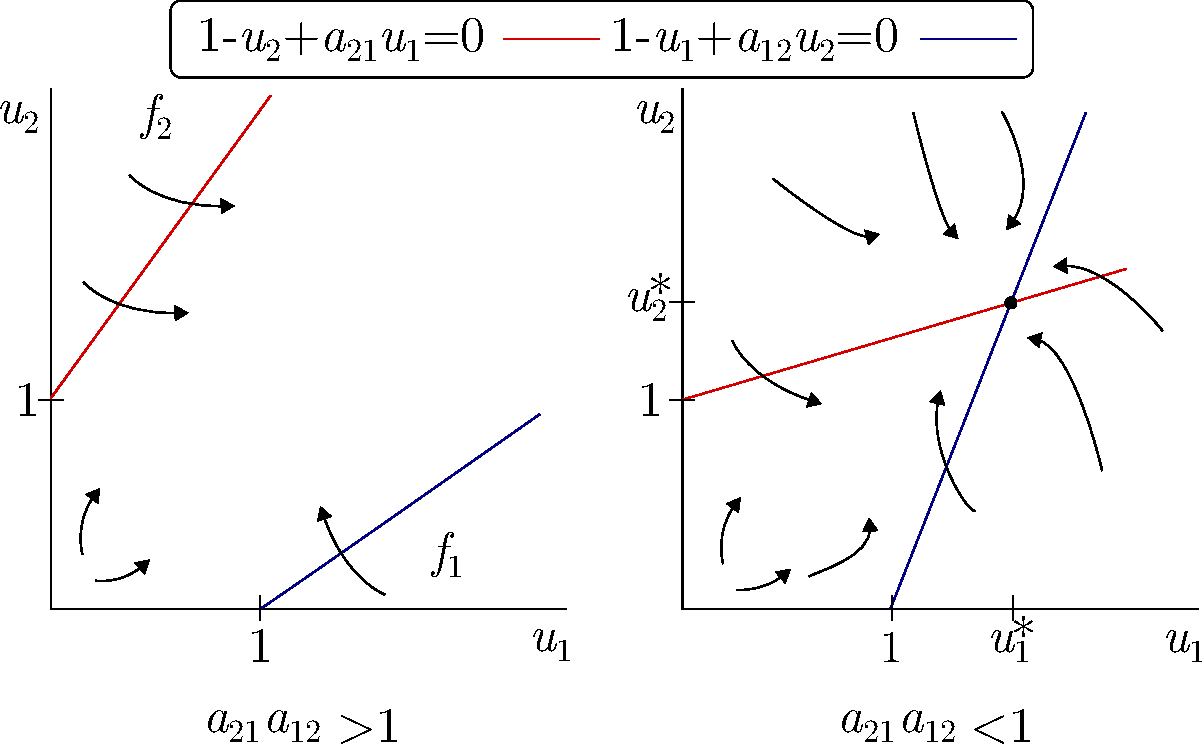
\includegraphics[width=0.5\textwidth]{figuras/equilibrio.pdf}
    \caption{Análisis gráfico del equilibrio del punto $P_4$. La flecha indica la dirección en la que crece la función.}
    \label{fig:mosquitos}
\end{figure}

%%%%%%%%%%%%%%%%%%%%%%%%%%%%%%%%%%%%%%%%%%%%%%%%%%%%%%%%%%

Para este punto es mas conveniente un análisis gráfico como el que puede verse en la Fig. \ref{fig:mosquitos}. El punto $P_4$ es la interseccion de las rectas roja y azul. Si $a_{12} a_{21} = 1$ las rectas son paralelas y no hay un punto de equilibrio. Si $a_{12} a_{21} > 1$ la interseccion de la recta y por tanto el punto de equilibrio queda fuera del rango del problema ($u_1$ y $u_2$ son poblaciones y por tanto positivas). Si $a_{12} a_{21} < 1$ El punto de equilibrio queda en el primer cuadrante del plano $u_1, u_2$. Como por arriba de la recta roja $f_2>0$ y por arriba de la recta azul $f_1>0$ la direccion de crecimiento es la que se indica en la figura. La flecha va de valores crecientes a decrecientes. Con este analisis es posible determinar que la interseccion de las rectas para $a_{12} a_{21} < 1$ es un nodo estable.

% 
% ███████╗██╗  ██╗    ██████╗  
% ██╔════╝╚██╗██╔╝    ╚════██╗
% █████╗   ╚███╔╝      █████╔╝
% ██╔══╝   ██╔██╗     ██╔═══╝ 
% ███████╗██╔╝ ██╗    ███████╗
% ╚══════╝╚═╝  ╚═╝    ╚══════╝

\section{Resolucion Ej 2:}

Para el sistema:

\begin{equation}\label{eq:esteril1}
    \frac{d N}{d t} = f(N,a,b,k,n) 
    = \left[\frac{a N}{N+n}-b\right] N- k N(N+n)
\end{equation}

donde $a$ es la natalidad, $b$ es la mortalidad y $k$ un coeficiente de capacidad. Y $n$ es la poblacion de mosquitos esteriles que se mantiene constante.

Este modelo cuenta con las siguientes suposiciones:

% We incorporated into our model(s) the following explicit assumptions that would seem to apply to a rather wide range of biological situations: 

\begin{enumerate}[label=\alph*)]
    \item Las poblaciones existen como continuos y se reproducen de forma continua en el tiempo.
    \item La población crece similar a una curva logística.
    \item La capacidad de carga de un ambiente es constante.
    \item Los machos estériles y no estériles compiten en pie de igualdad.
    \item El apareamiento es al azar, la proporción de apareamientos fértiles es directamente proporcional al número de individuos fértiles presentes en la población.
    % \item Ambos géneros son monogámicos o si las hembras se aparean es igual de posible que lo haga con un individuo fértil o uno no fértil.
    % \item En caso de que exista poligamia cada individuo se aparea un número aleatorio de veces. El número de eventos de apareamiento siguen una distribución Poisson con media idéntica para todos los individuos.
    \item Los géneros están en una razón 1 a 1 constantemente.
    \item La liberación de individuos estériles es continua y a un ritmo constante por unidad de tiempo y hábitat.
    \item La liberación lleva a la completa e instantánea mezcla de individuos.
\end{enumerate}

Para obtener la capacidad del sistema analizamos el caso en el que $n=0$. 

\begin{equation}\label{eq:esteril2}
    \frac{d N}{d t} = f(N,a,b,k,0) 
    = 
    rN(1-\frac{k}{r}N)
    , \text{con } r = a-b
\end{equation}

Esta es una ecuacion logistica modificada, la natalidad esta controlada por la porcion de mosquitos que son esteriles. Ademas que los mosquitos esteriles influyen en la capacidad del sistema. Como sabemos los puntos fijos de un sistema logistico son, 0 y la capacidad del sistema, de esto puede verse de que $\frac{a-b}{k}$ es la capacidad del sistema.

Volviendo a Ec. \ref{eq:esteril1} los puntos fijos dados por: $f(N,a,b,k,n) = 0$

% $$
% \Nstar_1 = 0, 
% \Nstar_{2,3} = \frac{1}{2k} 
% \left( 
%     \pm \sqrt{(b-a)^2 - 4 a k n} + 
%     a - 2kn - b
% \right)
% $$

$$
\Nstar_1 = 0, 
\Nstar_{2,3} = \pm 
\sqrt{
    \frac{1}{4} \left( \frac{a-b}{k} \right)^2 - a n 
    }
+ \frac{a-b}{2k} 
- n
$$

Para anlizar la estabilidad de los puntos fijos, analizamos $\frac{d f}{d N}$:

$$
\frac{d f}{d N} = - b + \frac{ aN^2 + 2 a n N}{( N + n )^2}
- k (2N + n)
$$

La estabilidad de $\Nstar_1$:

$$
\frac{d f}{d N} = - b - k  n \Rightarrow  \Nstar_1 \text{ Es estable}
$$

La estabilidad de los puntos $\Nstar_{2,3}$ es un tanto mas complicada, pero podemos analizar bajo que condiciones estos puntos fijos desaparecen (se vuelven valores complejos).

$$
n_c =  
\frac{1}{4} 
\frac{k}{a} 
\left( \frac{a-b}{k} \right)^2 = n 
$$

Donde, reordenando, vemos que $n_c$ es menor que $ \frac{1}{4} $ de la capacidad:

$$
n_c =  
\underbrace{\frac{a-b}{a} }_{<1}
\frac{1}{4} 
\underbrace{\left( \frac{a-b}{k} \right)}_{Capacidad }
$$

%%%%%%%%%%%%%%%%%%%%%%%%%%%%%%%%%%%%%%%%%%%%%%%%%%%%%%%%%%%%%%%%%%%%%%
\sepline
%%%%%%%%%%%%%%%%%%%%%%%%%%%%%%%%%%%%%%%%%%%%%%%%%%%%%%%%%%%%%%%%%%%%%%

Con Ec. \ref{eq:esteril1} en cuenta puede plantearse un sistema en el que se suelte una unica vez a los mosquitos esteriles.

\begin{equation}
    \left\lbrace
    \begin{aligned}
        \frac{d n}{d t}&=  -b n - k (N+n) n \\
        \frac{d N}{d t}&=\left[\frac{a N}{N+n}-b\right] N- k N(N+n)
    \end{aligned}
    \right. ,
\end{equation}

Para la Ec. \ref{eq:esteril1}  $a$ es la natalidad, $b$ es la mortalidad y $k$ un coeficiente de capacidad. Con esto en cuenta puede plantearse un sistema en el que se suelte una unica vez a los mosquitos esteriles.

Son 3 puntos de equilibrios $P_j = (\nstar_{j},\Nstar_{j}), j= 1, 2, 3$.

El origen es un punto estable, la derivada se anula en ese punto y no hay dinamica.

$$
\begin{aligned}
    P_1 &= (0, 0) , &P_2 &= \left( 0, \frac{a-b}{k} \right) \\ 
    P_3 &= \left(- \frac{b}{k}, 0 \right) \left(^\text{Población}_\text{Negativa} \right) ,  &P_4 &= \left(- \frac{b}{k}, \frac{b+a}{k} \right) \left(^\text{Población}_\text{Negativa} \right)
\end{aligned}
$$

% $$
% J = 
% \begin{bmatrix}
%     -2kx-ky-b & -kx \\
%     \frac{-ky^2-2kyx-ay-kx^2}{\left(y+x\right)^2} & \frac{-kx^2+ax-2kyx-ky^2}{\left(y+x\right)^2}
% \end{bmatrix}
% $$

% $$
% J_1 = 
% \begin{bmatrix}
%     -b & 0 \\
%     0 & 0
% \end{bmatrix}
% $$

$$
J_2 = 
\begin{bmatrix}
    -a & 0  \\
    k \frac{b - 2a}{ a - b } & -k 
\end{bmatrix}
\Rightarrow  P_2 \ \text{Estable}
$$

El punto $P_3$ no forma parte de la dinamica (No hay poblaciones negativas)

% $$
% J_3 = 
% \begin{bmatrix}
%     b & b \\
%     -k &  - k \frac{ b+a}{ b }
% \end{bmatrix}
% $$

Donde puede verse que no se puede llegar a la extinción mediante este método de liberación.

%%%%%%%%%%%%%%%%%%%%%%%%%%%%%%%%%%%%%%%%%%%%%%%%%%%%%%%%%%%%%%%%%%%%%%
\sepline
%%%%%%%%%%%%%%%%%%%%%%%%%%%%%%%%%%%%%%%%%%%%%%%%%%%%%%%%%%%%%%%%%%%%%%

Si se propone que una fraccion $\gamma$ de los mosquitos nace esteriles se tiene que:

\begin{equation}
    \left\lbrace
    \begin{aligned}
        \frac{d n}{d t}&=  \gamma N - b n
        \\
        \frac{d N}{d t}&=\left[\frac{a N}{N+n}-b\right] N- k N(N+n) 
    \end{aligned}
    \right. ,
\end{equation}

% \begin{figure}[!ht]
%     \centering
%     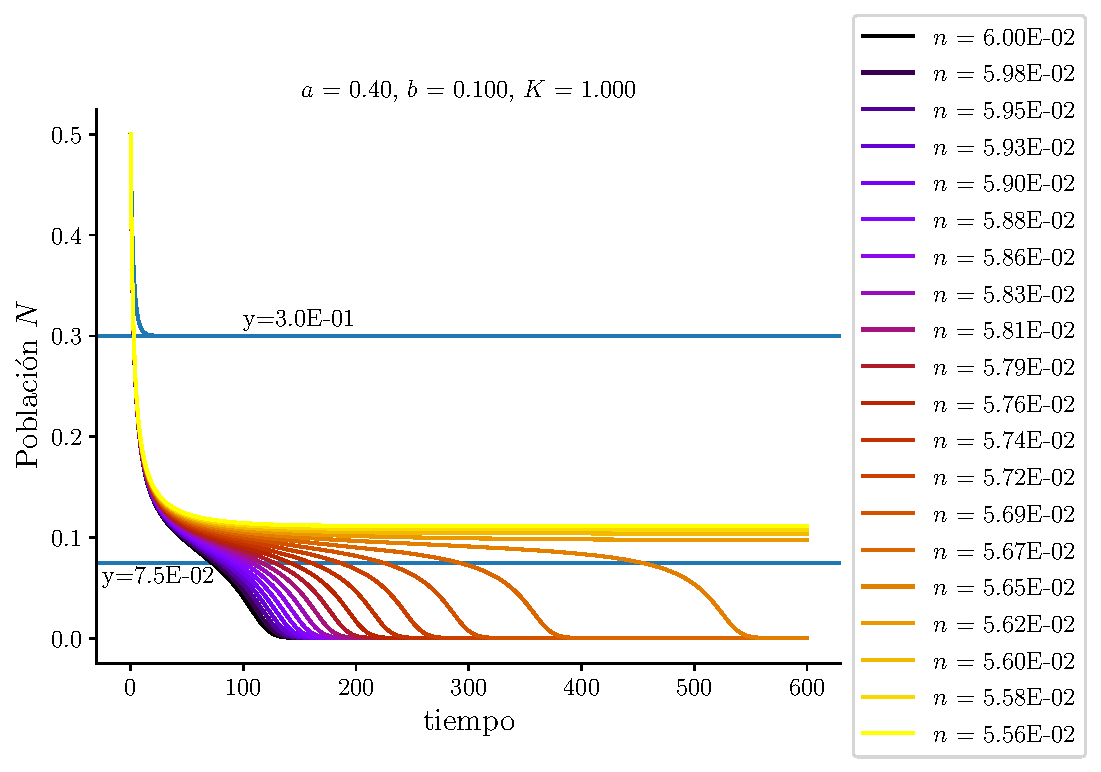
\includegraphics[width=0.51\textwidth]{figuras/ex02.pdf}
%     \caption{Evolucion de los mosquitos fertiles para distintos valores de los mosquitos esteriles.}
%     \label{fig:esteriles}
% \end{figure}

% En la Fig. \ref{fig:esteriles} pueden verse graficos de la resolucion numerica del sistema para distintos valores de el parametro $n$.


$$
\begin{aligned}
    P_1 &= (0, 0) ,\\
    P_2 &= \left( \frac{\gamma}{b} \left( \tusa \right), \left( \tusa \right) \right), \\ 
\end{aligned}
$$

% $$
% J = 
% \begin{bmatrix}
%     -2kx-ky-b & -kx \\
%     \frac{-ky^2-2kyx-ay-kx^2}{\left(y+x\right)^2} & \frac{-kx^2+ax-2kyx-ky^2}{\left(y+x\right)^2}
% \end{bmatrix}
% $$


% $$
% J_1 = 
% \begin{bmatrix}
%     -b & \gamma \\
%     \frac{-k(0)^2-2k(0)(0)-a(0)-k(0)^2}{\left((0)+(0)\right)^2} & \frac{-k(0)^2+a(0)-2k(0)(0)-k(0)^2}{\left((0)+(0)\right)^2}
% \end{bmatrix}
% $$


% $$
% J_2 = 
% \begin{bmatrix}
%     -b & \gamma \\
%     \frac{-k(N)^2-2k(N)(\frac{\gamma}{b} N)-a(N)-k(\frac{\gamma}{b} N)^2}{ N^2 \left( 1 + \frac{\gamma}{b} \right)^2} & \frac{-k(\frac{\gamma}{b} N)^2+a(\frac{\gamma}{b} N)-2k(N)(\frac{\gamma}{b} N)-k(N)^2}{ N^2 \left( 1 + \frac{\gamma}{b} \right)^2}
% \end{bmatrix}
% $$

% $$
% J_2 = 
% \begin{bmatrix}
%     -b & \gamma \\
%     -k \frac{(2a-(b+\gamma)}{a-(b+\gamma)} & \frac{-k(\frac{\gamma}{b} N)^2+a(\frac{\gamma}{b} N)-2k(N)(\frac{\gamma}{b} N)-k(N)^2}{ N^2 \left( 1 + \frac{\gamma}{b} \right)^2}
% \end{bmatrix}
% $$

% $$
% J_2 = 
% \begin{bmatrix}
%     -b & \gamma \\
%     -k \frac{2a-(b+\gamma)}{a-(b+\gamma)} & -k \frac{a (1 - \frac{\gamma}{b}) -(b+\gamma)}{a-(b+\gamma)}
% \end{bmatrix}
% $$

Para que con este modelo la extincion sea inevitable, es decir, tengamos un unico nodo estable en el origen. Se requiere que $\gamma = a-b$. En este caso se pierde el segundo punto fijo.

% We incorporated into our model(s) the following explicit assumptions that would seem to apply to a rather wide range of biological situations: 

% \begin{enumerate}[label=\alph*)]
%     \item Las poblaciones existen como continuos y se reproducen de forma continua en el tiempo.
%     \item La población crece similar a una curva logística.
%     \item La capacidad de carga de un ambiente es constante.
%     \item Los machos estériles y no estériles compiten en pie de igualdad.
%     \item El apareamiento es al azar, la proporción de apareamientos fértiles es directamente proporcional al número de individuos fértiles presentes en la población.
%     % \item Ambos géneros son monogámicos o si las hembras se aparean es igual de posible que lo haga con un individuo fértil o uno no fértil.
%     % \item En caso de que exista poligamia cada individuo se aparea un número aleatorio de veces. El número de eventos de apareamiento siguen una distribución Poisson con media idéntica para todos los individuos.
%     \item Los géneros están en una razón 1 a 1 constantemente.
%     \item La liberación de individuos estériles es continua y a un ritmo constante por unidad de tiempo y hábitat.
%     \item La liberación lleva a la completa e instantánea mezcla de individuos.
% \end{enumerate}

% 
% ███████╗██╗  ██╗    ██████╗     
% ██╔════╝╚██╗██╔╝    ╚════██╗    
% █████╗   ╚███╔╝      █████╔╝    
% ██╔══╝   ██╔██╗      ╚═══██╗    
% ███████╗██╔╝ ██╗    ██████╔╝    
% ╚══════╝╚═╝  ╚═╝    ╚═════╝     
%                                 
% 

\section{Resolucion Ej 3:}

Para el siguiente sistema de competencia ciclica:
$$
\left\{
\begin{aligned}
\frac{d n_{1}}{d t}&=n_{1}\left(1-n_{1}-\alpha n_{2}-\beta n_{3}\right) = f_1(n_1,n_2,n_3)\\
\frac{d n_{2}}{d t}&=n_{2}\left(1-\beta n_{1}-n_{2}-\alpha n_{3}\right) = f_2(n_1,n_2,n_3) \\
\frac{d n_{3}}{d t}&=n_{3}\left(1-\alpha n_{1}-\beta n_{2}-n_{3}\right) = f_3(n_1,n_2,n_3)
\end{aligned}
\right.
$$
con $0<\beta<1<\alpha$ y $\alpha+\beta>2$. Pueden obtenerse los  equilibrios viendo todos los puntos que cumplan simultaneamente: 

\begin{itemize}\centering
    \item[] 
    $\left\lbrace
    \begin{aligned}
        f_1(\nstar_1,\nstar_2,\nstar_3) = 0\\ 
        f_2(\nstar_1,\nstar_2,\nstar_3) = 0\\ 
        f_3(\nstar_1,\nstar_2,\nstar_3) = 0   
    \end{aligned}\right.
    $
\end{itemize}


Son 8 puntos de equilibrios $P_j = (\nstar_{1,j},\nstar_{2,j},\nstar_{3,j}), j= 1, 3, ..., 8$.

$$
\begin{aligned}
    P_1 &= (0, 0, 0) \\ 
    P_2 &= (1, 0, 0), P_3 = (0, 1, 0), P_4 = (0, 0, 1) \\
    P_5 &= \frac{1}{\alpha \beta - 1} 
                       (\alpha - 1, \beta - 1 , 0)  \left(^\text{Población}_\text{Negativa} \right)  \\ 
    P_6 &= \frac{1}{\alpha \beta - 1} 
                       (0         , \alpha - 1, \beta - 1)  \left(^\text{Población}_\text{Negativa} \right)  \\ 
    P_7 &= \frac{1}{\alpha \beta - 1} 
                       (\beta - 1 , 0         , \alpha - 1)  \left(^\text{Población}_\text{Negativa} \right)  \\ 
    P_8 &= \frac{1}{\alpha + \beta + 1}(1, 1, 1) 
\end{aligned}
$$

Analizamos el la matriz jacobiana de este sistema:

$$
\mathbf{J}_1 = 
\begin{bmatrix}
    1  & 0 & 0 \\
    0 & 1 & 0 \\
    0 & 0 & 1
\end{bmatrix} (\text{estable})
\quad 
\mathbf{J}_8 = 
\frac{1}{1+\alpha+\beta}\begin{bmatrix}
    -1 & -\alpha & -\beta \\
    -\beta & -1 & -\alpha \\
    -\alpha & -\beta & -1
\end{bmatrix}
$$

$$
\mathbf{J}_2 = 
\begin{bmatrix}
    -1 & - \alpha & - \beta \\
    0 & 1-\beta & 0 \\
    0 & 0 & 1- \alpha
\end{bmatrix} (\text{Punto silla})
$$

$$
\mathbf{J}_3 = 
\begin{bmatrix}
    1 - \alpha  & 0 & 0 \\
    - \beta & -1 & - \alpha \\
    0 & 0 & 1  - \beta
\end{bmatrix} (\text{Punto silla})
$$

$$
\mathbf{J}_4 = 
\begin{bmatrix}
    1 - \beta  & 0 & 0 \\
    0 & 1 -\alpha  & 0 \\
    - \alpha  & -\beta & -1
\end{bmatrix} (\text{Punto silla})
$$

% $$
% \mathbf{J}_5 = 
% \begin{bmatrix}
%     -\talf  & - \alpha (\talf)& - \beta (\talf)\\
%     - \beta (\tbet) & -\tbet & - \alpha (\tbet) \\
%     0 & 0 & 1 - \alpha (\talf) - \beta (\tbet)
% \end{bmatrix}
% $$

% $$
% \mathbf{J}_6 = 
% \begin{bmatrix}
%     1 - \alpha (\talf) - \beta (\tbet) & 0 & 0 \\
%     - \beta (\talf) & -\talf & - \alpha (\talf) \\
%     - \alpha (\tbet) & - \beta (\tbet) & \tbet
% \end{bmatrix}
% $$

% $$
% \mathbf{J}_7 = 
% \begin{bmatrix}
%     -\tbet & - \alpha (\tbet) & - \beta (\tbet) \\
%     0 & 1 - \beta (\tbet) - \alpha (\talf) & 0 \\
%     - \alpha (\talf) & - \beta (\talf) & \talf
% \end{bmatrix}
% $$

$P_5, P_6, P_7$ no es accesible en el modelo porque son valores negativos y se estan tratando poblaciones.

El origen es equilibrio (una fuente) y los versores $(1,0,0)$ etc. son puntos de ensilladura. Hay otros 3 equilibrios con dos poblaciones finitas y una nula. Finalmente, existe un equilibrio interior al octante $\mathbb{R}_{+}^{3}$, dado por:
$$
x_{1}^{*}=x_{2}^{*}=x_{3}^{*}=\frac{1}{1+\alpha+\beta} .
$$
Este equilibrio de coexistencia es una ensilladura, lo cual se demuestra fácilmente porque los autovalores son muy sencillos. La matriz del sistema linealizado es "circulante":
$$
\frac{1}{1+\alpha+\beta}\left(\begin{array}{ccc}
-1 & -\alpha & -\beta \\
-\beta & -1 & -\alpha \\
-\alpha & -\beta & -1
\end{array}\right)
$$
con lo que sus autovalores son combinaciones de las raíces cúbicas de la unidad:
$$
\lambda_{k}=\sum_{j=0}^{n-1} c_{j} \gamma_{j}^{k}, \quad k=0,1, \ldots, n-1
$$
con $c_{j}$ los elementos de la matriz y $\gamma_{j}$ las raíces de la unidad, $\gamma_{j}=\exp (2 \pi i / n)$, en general. Así que:
$$
\begin{array}{c}
\lambda_{0}=-1, \text { con autovector }(1,1,1) \\
\lambda_{1}=\lambda_{2}^{*}=\frac{1}{1+\alpha+\beta}\left(-1-\alpha e^{2 x i / 3}-\beta e^{4 \pi i / 3}\right),
\end{array}
$$
que satisfacen:
$$
\operatorname{Re}\left(\lambda_{1}\right)=\operatorname{Re}\left(\lambda_{2}\right)=\frac{1}{1+\alpha+\beta}\left(-1+\frac{\overbrace{\alpha+\beta}^{>2}}{2}\right)>0
$$

% 
% ███████╗██╗  ██╗    ██╗  ██╗
% ██╔════╝╚██╗██╔╝    ██║  ██║
% █████╗   ╚███╔╝     ███████║
% ██╔══╝   ██╔██╗     ╚════██║
% ███████╗██╔╝ ██╗         ██║
% ╚══════╝╚═╝  ╚═╝         ╚═╝
%                             
% 

\section{Resolucion Ej 4:}

% El sistema de ecuaciones
% $$
% \left\{
% \begin{aligned}
% \frac{d x}{d t} = f_1(x, y, z) &=-c_{a} x y+e_{a} y-c_{b} x z+e_{b} z \\
% \frac{d y}{d t} = f_2(x, y, z) &=c_{a} x y-e_{a} y+c_{a} z y          \\
% \frac{d z}{d t} = f_3(x, y, z) &=c_{b} x z-e_{b} z-c_{a} z y            
% \end{aligned}
% \right.
% $$

% Los equilibrios vienen dados por 

% $$
% \left\{
% \begin{aligned}
%     f_1(x^*, y^*, z^*) &= 0\\ 
%     f_2(x^*, y^*, z^*) &= 0\\ 
%     f_3(x^*, y^*, z^*) &= 0\\
%     x^* + y^* + z^* &= h
% \end{aligned}
% \right.
% $$

% Por esto los puntos fijos son:

% % $$
% % \begin{aligned}
% %     P_1 &= (0, 0, 0) \\ 
% %     P_2 &= (\frac{e_b}{c_b}, 0, z) \\ 
% %     P_3 &= (\frac{e_a}{c_a}, y, 0) \\ 
% %     P_4 &= (\frac{e_a}{c_a} - c_a z, z, \frac{c_b}{c_a} (\frac{e_a}{c_a} - c_a z) - \frac{e_b}{c_a}) 
% % \end{aligned}
% % $$

% $$
% \begin{aligned}
%     P_1 &= (0, 0, 0) \\ 
%     P_2 &= (\frac{e_b}{c_b}, 0, h - \frac{e_b}{c_b}) \\ 
%     P_3 &= (\frac{e_a}{c_a}, h - \frac{e_a}{c_a}, 0) \\ 
%     P_4 &= (\frac{e_a}{c_a} - c_a z, z, \frac{c_b}{c_a} (\frac{e_a}{c_a} - c_a z) - \frac{e_b}{c_a}) 
% \end{aligned}
% $$

% $$
% J = 
% \begin{bmatrix}  
%     - y c_a - z c_b & - x c_a + e_a & - x c_b + e_b \\
%     y c_a & x c_a - e_a + z c_a & y c_a \\
%     z c_b & - z c_a & x c_b - e_b - y c_a 
% \end{bmatrix}
% $$

% $$
% J_1 = 
% \begin{bmatrix}
%     0 & e_a & e_b \\
%     0 & - e_a & 0 \\
%     0 & 0 & - e_b 
% \end{bmatrix}
% $$

% $$
% J_2 = 
% \begin{bmatrix}  
%     - z c_b & - (\frac{e_b}{c_b}) c_a + e_a & - (\frac{e_b}{c_b}) c_b + e_b \\
%     0 & (\frac{e_b}{c_b}) c_a - e_a + z c_a & 0 \\
%     z c_b & - z c_a & (\frac{e_b}{c_b}) c_b - e_b
% \end{bmatrix}
% $$


% $$
% J = 
% \begin{bmatrix}  
%     - y c_a & - (\frac{e_a}{c_a}) c_a + e_a & - (\frac{e_a}{c_a}) c_b + e_b \\
%     y c_a & (\frac{e_a}{c_a}) c_a - e_a  & y c_a \\
%     0 & 0 & (\frac{e_a}{c_a}) c_b - e_b - y c_a 
% \end{bmatrix}
% $$


%%%%%%%%%%%%%%%%%%%%%%%%%%%%%%%%%%%%%%%%%%%%%%%%%%%%%%%%%%%
%%%%%%%%%%%%%%%%%%%%%%%%%%%%%%%%%%%%%%%%%%%%%%%%%%%%%%%%%%%
%%%%%%%%%%%%%%%%%%%%%%%%%%%%%%%%%%%%%%%%%%%%%%%%%%%%%%%%%%%

Supongamos que se produce una fragmentación del hábitat y que hay parches que son inhabitables. 

Seguimos considerando competencia entre s e $i$. 

Pero ahora hay una fracción de zonas habitables $h<1$ 

$h \quad$ Fracción de zonas habitables 

$v=h-p_{s}-p_{i} \quad$ Fracción de zonas vacías 

$$
\left\{ 
    \begin{aligned}
        \frac{d p_{s}}{d t} = f_{s}(p) &= c_{s} p_{s}\left(h-p_{s}\right)-e_{s} p_{s} \\
        \frac{d p_{i}}{d t} = f_{i}(p) &= c_{i} p_{i}\left(h-p_{i}-p_{s}\right)-e_{i} p_{i}-c_{s} p_{i} p_{s}
    \end{aligned}
\right.
$$

$$
\left\{ 
    \begin{aligned}
        \frac{d p_{s}}{d t} = f_{s}(p) &= c_{s} p_{s}\left(v+p_{i}\right)+-e_{s} p_{s} \\
        \frac{d p_{i}}{d t} = f_{i}(p) &= c_{i} p_{i} v-e_{i} p_{i}-c_{s} p_{i} p_{s}=f_{i}(p)
    \end{aligned}
\right.
$$

$$
\frac{d v}{d t}=e_{i} p_{i}+e_{s} p_{s}-v\left(c_{s} p_{s}+c_{i} p_{i}\right)
$$

$$
\begin{aligned}
    \frac{d p_{s}}{d t} &= c_{s} p_{s}\left(h-p_{s}\right)-e_{s} p_{s} \\
    \frac{d p_{i}}{d t} &= c_{i} p_{i}\left(h-p_{i}-p_{s}\right)-e_{i} p_{i}-c_{s} p_{i} p_{s} \\
    \frac{d     v}{d t} &= e_{i} p_{i}+e_{s} p_{s}-v\left(c_{s} p_{s}+c_{i} p_{i}\right)
\end{aligned}
$$

$$
\left\{
\begin{array}{l}
    c_{s} p_{s}\left(h-p_{s}\right)-e_{s} p_{s}=0 \\
    c_{s}\left(h-p_{s}\right)-e_{s}=0
\end{array} 
\Rightarrow 
p_{s}^{*}=h-\frac{e_{s}}{c_{s}}
\right.
$$

\begin{equation}
    \left\{
    \begin{array}{l}
    c_{i} p_{i}\left(h-p_{i}-p_{s}\right)-e_{i} p_{i}-c_{s} p_{i} p_{s}=0 \\
    c_{i}\left(h-p_{i}-h+\frac{e_{s}}{c_{s}}\right)-e_{i}-c_{s}\left(h-\frac{e_{s}}{c_{s}}\right)=0 \\
    -c_{i} p_{i}-\frac{c_{i} e_{s}}{c_{s}}-e_{i}-c_{s} h+e_{s}=0
    \end{array}
    \right.
\end{equation}

\begin{equation}
    \left\{\begin{array}{l}
    p_{s}^{*}=h-\frac{e_{s}}{c_{s}} \\
    p_{i}^{*}=\frac{e_{s}\left(c_{s}+c_{i}\right)}{c_{s} c_{i}}-\frac{e_{i}}{c_{i}}-\frac{h c_{s}}{c_{i}} \\
    v^{*}=\frac{h c_{s}-e_{s}+e_{i}}{c_{i}}
    \end{array}\right.
\end{equation}

Vemos que cuando el valor de h está por debajo de $\mathrm{e}_{\mathrm{s} /} \mathrm{c}_{\mathrm{s}}$ la población de s se extingue. En ese caso, en ausencia de s, la población de $i$ puede persistir si
$$
\frac{c_{i}}{e_{i}}>\frac{c_{s}}{e_{s}}
$$
ya que en ese caso la ecuación para i es
$$
\frac{d p_{i}}{d t}=c_{i} p_{i}\left(h-p_{i}\right)-e_{i} p_{i}
$$

Los valores estacionarios muestran que cuando $h$ disminuye aumenta la población de $i $ y disminuye la de s. Las ventajas de $i$ surgen de una menor mortalidad o una mejor estrategia de colonización

% 
% ███████╗██╗  ██╗    ███████╗
% ██╔════╝╚██╗██╔╝    ██╔════╝
% █████╗   ╚███╔╝     ███████╗
% ██╔══╝   ██╔██╗     ╚════██║
% ███████╗██╔╝ ██╗    ███████║
% ╚══════╝╚═╝  ╚═╝    ╚══════╝
%                             
% 

\section{Resolucion Ej 5:}

Metapoblaciones - Modelo de Levins


$$\frac{d p}{d t}=c p(1-p)-e p = f(p)$$

\begin{itemize}
    \item $c:$ Tasa de colonización local de un parche (o probabilidad de que un parche vacío sea colonizado por individuos que migran al mismo parche desde parches ocupados). 
    \item $p:$ Fracción de parches ocupados
    \item $1-p:$ Fracción de parches vacíos
    \item $e:$ Tasa de extinción de cualquier subpoblación (población local en un parche) o probabilidad de que un parche ocupado quede vacío (extinción local).
\end{itemize}

Lo que parece un término logístico tiene un origen muy diferente. La posibilidad de que aumente la fracción de parches ocupados depende de cuantos parches hay ocupados y de la posibilidad de ocupar uno nuevo, que para eso, debe estar vacio. De ahí el producto de ambas cantidades

$$
f(p) = 0 \Rightarrow\left\{
\begin{array}{l}
    p=0 \\ 
    p=1-\frac{e}{c}
\end{array}
\right.
$$
Metapoblaciones - Competencia
Tenemos dos especies compitiendo, pero una de las dos (s) es mejor colonizadora y

$$
\left\{
\begin{aligned}
    \frac{d p_{s}}{d t} &=f_{s}(p)=c_{s} p_{s}\left(1-p_{s}\right)-e_{s} p_{s} \\ 
    \frac{d p_{i}}{d t} &=f_{i}(p)=c_{i} p_{i}\left(1-p_{i}-p_{s}\right)-e_{i} p_{i}-c_{s} p_{i} p_{s}
\end{aligned} 
\right.
$$

$$
\left\{
\begin{array} { l } 
    { f _ { i } = 0 } \\
    { f _ { s } = 0 }
\end{array} 
\right. 
\Rightarrow 
\left\{
\begin{array}{l}
    p_{i}=p_{s}=0 \\
    p_{i}=0, p_{s}=1-e_{s} / c_{s} \\
    p_{i}=1-e_{i} / c_{i}, p_{s}=0 \\
    p_{i}=p_{i}^{*}, p_{s}=p_{s}^{*}
\end{array}
\right.
$$



$$
p_{s}^{*}=1-\frac{e_{s}}{c_{c}}, p_{i}^{*}=1-p_{s}^{*}-\frac{e_{i}+c_{s} p_{s}^{*}}{c_{i}}
$$

$$
1 - \frac{e_{s}}{c_{s}} > 0
$$

\begin{equation}
    \mathbf{J}=\left(
    \begin{array}{cc}
        -c_{s}+e_{s} & 0 \\
        \frac{d f_{i}}{d p_{i}} & c_{i}\left(1-p_{s}^{*}-2 p_{i}^{*}\right)-e_{i}-c_{s} p_{s}^{*}
    \end{array}
    \right)
\end{equation}

Para que la coexistencia sea estable necesito dos autovalores negativos, es decir

$$
c_{i}\left(1-p_{s}^{*}-2 p_{i}^{*}\right)-e_{i}-c_{s} p_{s}^{*}<0
$$

$$
c_{i}>c_{s}\left(\frac{e_{i}}{e_{s}}+\frac{p_{s}^{*}}{1-p_{s}^{*}}\right) \quad c_{i}>c_{s}\left(\frac{c_{s}+e_{i}-e_{s}}{e_{s}}\right)
$$

Supongamos que los coeficientes de extinción son iguales. Si $p_{s}{ }^{*}<1$ vemos que

$$
c_{i}>c_{s}
$$

La coexistencia ocurre porque $s$ deja huecos ya sea porque coloniza peor o tiene una mayor tasa de extinción.

% \bibliography{sample}

\end{document}

% ███    ██  ██████  ████████  █████  ███████
% ████   ██ ██    ██    ██    ██   ██ ██
% ██ ██  ██ ██    ██    ██    ███████ ███████
% ██  ██ ██ ██    ██    ██    ██   ██      ██
% ██   ████  ██████     ██    ██   ██ ███████


% ████████ ██    ██ ██████   ██████  ███████
%    ██     ██  ██  ██   ██ ██    ██ ██
%    ██      ████   ██████  ██    ██ ███████
%    ██       ██    ██      ██    ██      ██
%    ██       ██    ██       ██████  ███████

% A pesar de mis multiples y cultas intervenciones seguis escribiendo así, usa ctrl f y resolvelo.

% atomico
% volumen
% parametro
% mantenia
% dielectrico
% perdida
% ferroelectrico
% difractograma
% difractometro
% minimo
% maximo
% tension
% conversion
% aislacion
% medicion
% resolucion
% funcion
% transicion
% correccion
% activacion
% correlacion
% tipico X
% habia  X
% agrego X
